\documentclass{beamer}

\usepackage[francais]{babel}
\usepackage[utf8]{inputenc}
\usepackage[T1]{fontenc}
\usepackage{graphicx}
\usepackage{graphics}
\usepackage{color}
\usepackage{textcomp}
\usepackage{pifont}
\usepackage[normalem]{ulem}
\usepackage{times}
\usepackage{hyperref}
\usepackage{verbatim}
\usepackage{amsmath}
\usepackage{amsthm}
\usepackage{amsfonts}
\usepackage[mathscr]{euscript}
\usepackage{pgfpages}
\usepackage{listings}
\usepackage{subfigure}
\usepackage{algorithm}
\usepackage[noend]{algorithmic}
\usepackage{pdftricks}
\usepackage{mathrsfs}
\usepackage{array}
\usepackage{fancybox}
% \usepackage{columns}
\usepackage{multirow}
\usepackage{url}
\usepackage{tikz}
\usepackage{colortbl}
%\usepackage{cite} %DO NOT FUCKING USE CITE ON BEAMER !!! LOST 30 GODDAM' MINUTES ON THIS SHIT !!!
\usepackage{mathabx}
\usepackage{amssymb}
\usepackage{eurosym}
\usepackage{wasysym} % ch0

\let\texteuro\euro

\hypersetup{colorlinks,%
            citecolor=black,%
            filecolor=black,%
            linkcolor=black,%
            urlcolor=blue}

%\addtolength{\parskip}{10pt}

\usetikzlibrary{calc}

\mode<presentation>
\setbeamertemplate{footline}[frame number]
\setbeamercovered{transparent}
\usetheme[navigation]{ESI}

%lst
\definecolor{comment-green}{RGB}{0,166,80}
\lstset{language=C++,
  keywordstyle=\lst@ifdisplaystyle\bf\fi\color{blue!60},
  commentstyle=\color{comment-green},
  stringstyle=\color{red},
  basicstyle=\lst@ifdisplaystyle\tiny\else\tt\fi,
  morekeywords={
    constexpr,concept,decltype,nullptr,nullptr_t,noexcept,final,override},
  frame=single,
  xleftmargin=0.5cm,
  numbers=left,
  tabsize=2}

%title
\subtitle{Langage \texttt{C} / \cpp}
\author{R. Absil}
\date{\today}

%styles
\theoremstyle{definition}
\newtheorem{thm}{Théorème}
\newtheorem{conj}[thm]{Conjecture}
\newtheorem{deff}[thm]{Définition}
\newtheorem{prop}[thm]{Propriété}
\newtheorem{lem}[thm]{Lemme}
\newtheorem*{lem*}{Lemme}
\newtheorem{cor}[thm]{Corollaire}
%\newtheorem{example}{Exemple}
\newtheorem{remark}{Remarque}
\newtheorem{exo}{Exercice}

%typeset
\newcommand{\ie}{{\emph{i.e., }}}
\newcommand{\eg}{{\emph{e.g., }}}
\newcommand{\etal}{{\emph{et al.}}}
\newcommand{\rrceil}{\unichar{"2308}}
\newcommand{\sloand}[2]{\footnote{N. J. A. Sloane - OEIS Foundation - \texttt{www.oeis.org}, Sequence #1 - #2.}}

%math
\newcommand{\IN}{{\mathbb N}}
\newcommand{\IQ}{{\mathbb Q}}
\newcommand{\IR}{{\mathbb R}}
\newcommand{\IZ}{{\mathbb Z}}
\newcommand{\IP}{{\mathbb P}}
\newcommand{\IC}{{\mathbb C}}
\newcommand{\bigo}{{\mathcal{O}}}
\renewcommand{\mod}{\bmod}
\newcommand{\ssi}{\Leftrightarrow}
\newcommand{\then}{\Rightarrow}
\newcommand{\fle}[1]{\stackrel{#1}{\longrightarrow}}
\newcommand{\suchthat}{~\big|~}
\newcommand{\floor}[1]{\left\lfloor #1 \right\rfloor}
\newcommand{\ceil}[1]{\left\lceil #1 \right\rceil}
\DeclareMathOperator*{\argmin}{argmin}
\DeclareMathOperator*{\argmax}{argmax}

%tikz
\tikzstyle{_vertex}=[fill=white, circle,minimum size=12pt,inner sep=1pt]
\tikzstyle{_blackv}=[fill=black, circle,minimum size=8pt,inner sep=1pt]
\tikzstyle{_dot}=[fill=black, circle, minimum size = 1mm, inner sep=0pt]
\tikzstyle{_bigvertex}=[fill=white, circle,minimum size=21pt,inner sep=1pt]
\tikzstyle{_arc}=[->, >=stealth]
\tikzstyle{_boldarc}=[->, >=stealth, line width=2pt]

\newcommand{\cpp}{\texttt{C++}}
\newcommand{\java}{\texttt{Java}}


\title{Ch. 8 - Surcharge d'opérateur}

\begin{document}
\begin{frame}
  \titlepage
\end{frame}

\begin{frame}
  \frametitle{Table des matières}
  \footnotesize \tableofcontents[pausesections,pausesubsections]
\end{frame}


\section{Introduction}

\begin{frame}
\frametitle{Overview (1/2)}
\begin{itemize}[<+->]
\item \cpp\ autorise la surdéfinition de fonctions
	\begin{itemize}
	\item Fonctions membres
	\item Fonctions indépendantes
	\end{itemize}
\item Les opérateurs sont des fonctions comme les autres
\end{itemize}
\begin{exampleblock}<+->{Idée}
	\begin{itemize}[<+->]
	\item Surdéfinir certains opérateurs
	\item \texttt{a + b} doit être interprété correctement si \texttt{a} et \texttt{b} sont des vecteurs, par exemple
	\end{itemize}
\end{exampleblock}
\begin{itemize}[<+->]
\item Ce comportement existe déjà au sein du langage avec \texttt{+}
	\begin{itemize}
	\item Addition entière
	\item Addition flottante
	\end{itemize}
\end{itemize}
\end{frame}

\begin{frame}
\frametitle{Overview (2/2)}
\begin{columns}
	\begin{column}{.45\textwidth}
	\begin{itemize}[<+->]
	\item Autre exemple : \texttt{*}
		\begin{itemize}
		\item Multiplication
		\item Indirection
		\end{itemize}
	\end{itemize}
	\end{column}
	\begin{column}{.45\textwidth}
		\begin{itemize}[<+->]
		\item Autre exemple : \texttt{<<}
			\begin{itemize}
			\item Décalage de bits
			\item Impression console
			\end{itemize}
		\end{itemize}
		\end{column}
\end{columns}
\begin{itemize}[<+->]
\item La surcharge d'opérateur permet de donner de nouvelles interprétations d'opérateurs \emph{existants}
\item Syntaxe opératoire « plus claire » que syntaxe fonctionnelle
\end{itemize}
\begin{exampleblock}<+->{Exemple}
	\begin{itemize}[<+->]
	\item \lstinline|int a = add(b,c);|
	\item \lstinline|int a = b.add(c);|
	\item \lstinline|int a = b + c;|
	\end{itemize}
\end{exampleblock}
\begin{itemize}[<+->]
\item Parfois, la surcharge d'opérateur est indispensable
\end{itemize}
\end{frame}

\section{Contraintes}

\begin{frame}
\frametitle{Règles de base (1/2)}
\begin{exampleblock}<+->{Idée}
	\begin{itemize}[<+->]
	\item On ne peut pas changer la grammaire du \cpp
	\end{itemize}
\end{exampleblock}
\begin{itemize}[<+->]
\item Impossible de définir un nouvel opérateur
	\begin{itemize}
	\item \texttt{a § b} est interdit
	\item \texttt{a]b[} est interdit
	\end{itemize}
\item L'arité doit être respectée
	\begin{itemize}
	\item \texttt{a ++ b} est interdit
	\end{itemize}
\item Les priorités, associativités ne peuvent être changées
	\begin{itemize}
	\item \texttt{i + j * k} est toujours interprété comme \texttt{i + (j * k)}
	\item \texttt{i + j + k} est toujours interprété comme \texttt{(i + j) + k}
	\end{itemize}
\item Pas de commutativité par défaut
	\begin{itemize}
	\item Surdéfinir \texttt{+} entre une classe \texttt{A} et une classe \texttt{B} ne surdéfinit pas \texttt{+} entre une classe \texttt{B} et une classe \texttt{A}
	\end{itemize}
\end{itemize}
\end{frame}

\begin{frame}
\frametitle{Règles de base (2/2)}
\begin{itemize}[<+->]
\item Pas d'implication de signification
	\begin{itemize}
	\item Redéfinir \texttt{+} et \texttt{=} ne redéfinit ni \texttt{+=} ni \texttt{++}
	\end{itemize}
\item Certains opérateurs ont une signification par défaut
	\begin{itemize}
	\item Ils existent sur tous les types « classe »
	\item S'ils ne sont pas redéfinis, ils ont cette signification
	\item Exemple : \texttt{.}, \texttt{=}, \texttt{->}, etc.
	\end{itemize}
\item Les opérateurs \texttt{++} et \texttt{--} se comportent différemment
	\begin{itemize}
	\item Selon qu'ils soient préfixés ou suffixés
	\end{itemize}
\item Les opérateurs \lstinline|new| et \lstinline|delete| ont des paramètres fixés
	\begin{itemize}
	\item Nombre de bytes à allouer
	\item Mémoire à libérer
	\item Peuvent être définis
		\begin{enumerate}
		\item localement pour un type en particulier
		\item globalement pour tous les types
		\end{enumerate}
	\end{itemize}
\item L'évaluation paresseuse ne fonctionne pas pour \texttt{\&\&} et \texttt{||} surchargés
\end{itemize}
\end{frame}

\begin{frame}
\frametitle{Nécessité de classe}
\begin{itemize}[<+->]
\item Un opérateur redéfini doit comporter au moins un argument de type classe
	\begin{enumerate}
	\item Fonction membre : au moins le paramètre implicite \lstinline|this|
		\begin{itemize}
		\item Si opérateur unaire : pas d'autre argument
		\item Sinon, paramètre explicite
		\end{itemize}
	\item Fonction indépendante : un paramètre explicite pour chaque opérande
	\end{enumerate}
\end{itemize}
\begin{alertblock}<+->{Conséquence}
	\begin{itemize}[<+->]
	\item Impossible de redéfinir un opérateur pour les types de base
		\begin{itemize}
		\item Sauf \lstinline|new| et \lstinline|delete|
		\end{itemize}
	\end{itemize}
\end{alertblock}
\end{frame}

\begin{frame}
\frametitle{Bonnes pratiques}
\begin{itemize}[<+->]
\item On peut donner n'importe quelle signification à un opérateur
	\begin{itemize}
	\item Paramètres, retour, corps, etc.
	\end{itemize}
\end{itemize}
\begin{block}<+->{Hygiène de programmation}
	\begin{itemize}[<+->]
	\item Donner une signification « intuitive »	
	\end{itemize}
\end{block}
\begin{itemize}[<+->]
\item On s'attend à ce que \texttt{+} entre deux vecteurs définisse l'addition, et que ce soit commutatif
\item On s'attend à ce que \texttt{*} préfixé sur un itérateur retourne la donnée pointée
\end{itemize}
\end{frame}

\section{Surcharge d'opérateur}

\begin{frame}
\frametitle{Syntaxe}
\begin{itemize}[<+->]
\item Utilisation du mot-clé \lstinline|operator|
\item Deux utilisation possibles
	\begin{enumerate}
	\item Fonction membre
	\item Fonction indépendante (souvent amie)
	\end{enumerate}
\end{itemize}
\begin{exampleblock}<+->{Exemple : classe \texttt{fraction}}
	\begin{itemize}[<+->]
	\item Multiplication commutative avec \texttt{*}
		\begin{itemize}
		\item Membre
		\item Tous les opérandes sont de type \texttt{fraction}
		\end{itemize}	
	\end{itemize}
\end{exampleblock}
\begin{itemize}[<+->]
\item Ici, l'impression console est effectuée avec une fonction \texttt{toString}
	\begin{itemize}
	\item Mauvaise pratique
	\item Bonne pratique : surcharger \texttt{<<} (cf. section suivante)
	\end{itemize}
\end{itemize}
\end{frame}

\begin{frame}[containsverbatim]
\frametitle{Exemple}
\begin{itemize}
\item Fichier \texttt{fraction.cpp}
\end{itemize}
\begin{lstlisting}
class fraction
{
	unsigned num, denom;
	bool positive;

	public:
		fraction(int num = 0, int denom = 1);
		fraction(unsigned num, unsigned denom, bool positive);

		fraction operator *(fraction f) const; //member
		//friend fraction operator *(fraction f1, fraction f2); //indep
};
\end{lstlisting}
\begin{itemize}
\item La multiplication est définie comme fonction membre
	\begin{itemize}
	\item Un opérande implicite : \lstinline|this|
	\item Un opérande explicite : \texttt{f}
	\end{itemize}
\item La multiplication est définie comme fonction indépendante
	\begin{itemize}
	\item Deux opérandes explicites : \texttt{f1} et \texttt{f2}
	\item Permet de préserver la symétrie avec types primitifs
		\begin{itemize}
		\item Cf. Ch. 10 dédié aux conversions
		\end{itemize}
	\end{itemize}
\end{itemize}
\end{frame}

\begin{frame}[containsverbatim]
\frametitle{Exemple avec opérateur \texttt{*} membre}
\begin{itemize}
\item Fichier \texttt{fraction.cpp}
\end{itemize}
\begin{lstlisting}
fraction::fraction(int num, int denom) 
	: num(abs(num)), denom(abs(denom)), 
	positive((num >= 0 && denom >= 0) || (num <= 0 && denom <= 0))
{}

fraction::fraction(unsigned num, unsigned denom, bool positive) 
	: num(num), denom(denom), positive(positive)
{}

fraction fraction::operator *(fraction f) const
{
	return fraction(num * f.num, denom * f.denom, //overflow unsafe, use gcd and lcm
		(positive && f.positive) || (!positive && !f.positive));
}
\end{lstlisting}
\end{frame}

\begin{frame}[containsverbatim]
\frametitle{Exemple avec opérateur \texttt{*} indépendant}
\begin{itemize}
\item Fichier \texttt{fraction.cpp}
\end{itemize}
\begin{lstlisting}
class fraction
{
	...

	public:
		...
		
		friend fraction operator *(fraction f1, fraction f2);		
};

fraction operator*(fraction f1, fraction f2)
{
	return fraction(f1.num * f2.num, f1.denom * f2.denom, //overflow unsafe 
		(f1.positive && f2.positive) || (! f1.positive && !f2.positive));
}
\end{lstlisting}
\end{frame}

\begin{frame}
\frametitle{Remarques}
\begin{itemize}[<+->]
\item Une instruction \texttt{f1 * f2 * f3}
	\begin{itemize}
	\item est évaluée comme \texttt{(f1 * f2) * f3} (langage)
	\item crée des objets temporaires
		\begin{itemize}
		\item Leur nombre dépend du compilateur
		\item Des passages par adresse de temporaires peuvent être « cachés »
		\end{itemize}	
	\end{itemize}
\item On peut savoir ce que le compilateur fait en réécrivant les constructeurs de recopie, par défaut, surcharger l'opérateur \texttt{\&}, etc.
\end{itemize}
\begin{block}<+->{Hygiène de programmation}
	\begin{itemize}[<+->]
	\item Définissez des opérateurs indépendants du compilateur
	\end{itemize}
\end{block}
\end{frame}

\begin{frame}
\frametitle{Liberté}
\begin{itemize}[<+->]
\item Les opérateurs sont des fonctions comme les autres	
\item Possibilité de 
	\begin{itemize}
	\item transmettre les opérandes par référence
		\begin{itemize}
		\item Utile si gros objets
		\end{itemize}
	\item transmettre le retour par référence
	\item allouer dynamiquement le retour (peu recommandé)
		\begin{itemize}
		\item Overhead si petits objets
		\item Gestion mémoire « complexe », cf. Ch. 5
		\end{itemize}
	\item protéger les arguments contre la modification avec \lstinline|const|
		\begin{itemize}
		\item N'a de sens que s'ils sont transmis par référence
		\end{itemize}
	\item les rendre constants (\lstinline|const| en fin de prototype)
	\item les rendre \lstinline|inline|
	\end{itemize}
\end{itemize}
\end{frame}

\section[Surch. div.]{Surcharges diverses}

\begin{frame}
\frametitle{Impression console}
\begin{itemize}[<+->]
\item Pour l'instant, l'impression console était effectuée via
	\begin{itemize}
	\item une fonction \texttt{print}
		\begin{itemize}
		\item Problème de couplage I/O
		\end{itemize}
	\item une fonction \texttt{toString}, avec \texttt{string}
		\begin{itemize}
		\item Inefficace
		\end{itemize}
	\end{itemize}
%\item En pratique, on surcharge l'opérateur \lstinline{<< (ostream\&, const MaClasse& brol)}
%	\begin{itemize}
%	\item Avec une fonction amie, indépendante
%	\end{itemize}
\begin{exampleblock}<+->{En pratique}
	\begin{itemize}[<+->]
	\item Surcharge de \texttt{ostream\& <<(ostream\&, const MaClasse\& brol)}
	\item Avec une fonction amie, indépendante
	\end{itemize}
\end{exampleblock}
\item Comme on transmet le paramètre par référence, on doit le déclarer \lstinline|const| si on souhaite autoriser certaines conversions
\item On retourne le résultat de l'impression par référence afin
	\begin{itemize}
	\item de pouvoir traiter les affectations multiples
	\item d'éviter d'appeler le constructeur de recopie (interdit)
	\end{itemize}
\end{itemize}
\end{frame}

\begin{frame}[containsverbatim]
\frametitle{Exemple}
\begin{itemize}
\item Fichier \texttt{point.cpp}
\end{itemize}
\begin{lstlisting}
class point
{
	double _x, _y;

	public:
		point(double x = 0, double y = 0) : _x(x), _y(y) {}

		inline double x() const { return _x; }
		inline double y() const { return _y; }

		friend ostream& operator << (ostream& out, const point& p);
};

ostream& operator << (ostream& out, const point& p)
{
	out << "(" << p._x << " , " << p._y << ")";
	return out;
}
\end{lstlisting}
\end{frame}

\begin{frame}
\frametitle{Opérateurs arithmétiques}
\begin{itemize}[<+->]
\item Cf. section précédente avec \texttt{*} (\texttt{fraction.cpp})
\end{itemize}
\begin{exampleblock}<+->{Membre vs indépendant}
	\begin{itemize}[<+->]
	\item Définir en membre \lstinline|A operator +(int a);| permet de faire
		\begin{itemize}
		\item \texttt{a + 2} 
		\item mais pas \texttt{2 + a}
		\end{itemize}
	\item En indépendant, cette possibilité existe
		\begin{itemize}
		\item Fournir deux implémentations
		\end{itemize}
	\item Autre possibilité pour les membres : conversions définies par l'utilisateur (cf. Ch. 10)
	\end{itemize}
\end{exampleblock}
\begin{itemize}[<+->]
\item Éviter la redondance (\texttt{+}, \texttt{+=}, symétrie, etc.)
	\begin{itemize}
	\item Définir une implémentation
	\item Les autres sont \lstinline|inline| et appellent la première
	\end{itemize}
\end{itemize}
\end{frame}

\begin{frame}[containsverbatim]
\frametitle{Exemple}
\begin{itemize}
\item Fichier \texttt{vector2d.cpp}
\end{itemize}
\begin{lstlisting}
class vector2d
{
    double _x, _y;
    
    public:
        vector2d(double x = 0, double y = 0) : _x(x), _y(y) {}                            
    
        vector2d& operator +=(const vector2d& v)
        {
            _x += v._x;
            _y += v._y;
            
            return *this;
        }
    
        friend vector2d operator + (vector2d v1, const vector2d& v2)
        {
            v1 += v2;
            return v1;
        }
    
        friend ostream& operator <<(ostream& out, const vector2d& v)
        {
            return out << "(" << v._x << " , " << v._y << ")";
        }
};
\end{lstlisting}
\end{frame}

\begin{frame}[containsverbatim]
\frametitle{Surcharge de \lstinline|[]|}
\begin{itemize}
\item Fichier \texttt{charset.cpp}
\end{itemize}
\begin{lstlisting}
class CharSet
{
	vector<pair<char,unsigned> > codes;

	public:		
		void update(char c, unsigned code)
		{
			int i = find(c);
			if(i == -1)
				codes.push_back(std::make_pair(c, code));
			else
				codes[i].second = code;
		}

		unsigned& operator[](char c)
		{
			int i = find(c);
			if(i == -1)
				throw std::out_of_range("Invalide char");
			else
				return codes[i].second;
		}

		...
};
\end{lstlisting}
\end{frame}

\begin{frame}
\frametitle{Remarques}
\begin{itemize}[<+->]
\item Transmettre le retour de l'opérateur par référence permet d'écrire des instructions telles que \lstinline|set['a'] = 12;|
	\begin{itemize}
	\item Car c'est une lvalue
	\end{itemize}
\item Si l'on veut empêcher ce comportement, mais toujours éviter les copies, on peut retourner un \lstinline|const|
\item Souvent, les deux implémentations sont fournies
	\begin{itemize}
	\item La variante \lstinline|const| est appelée sur les objets \lstinline|const|
	\end{itemize}
\item En général, la communauté préfère éviter de créer du code permettant d'utiliser \lstinline|[][]|
	\begin{itemize}
	\item Complexe		
	\item L'opérateur \lstinline|[]| est unaire
	\item Utiliser l'opérateur \lstinline|()| (arité variable)
	\end{itemize}
\end{itemize}
\end{frame}

\begin{frame}
\frametitle{Incrémentation et décrémentation}
\begin{itemize}[<+->]
\item Possibilité d'être utilisé en préfixé et en suffixé
\end{itemize}
\begin{exampleblock}<+->{Deux prototypes}
	\begin{enumerate}[<+->]
	\item Préfixé : \lstinline|A& operator ++()|
	\item Suffixé : \lstinline|A operator ++(int)| (paramètre ignoré)
	\end{enumerate}
\end{exampleblock}
\begin{itemize}[<+->]
\item Très utile pour l'itération avec une boucle \texttt{foreach}
	\begin{enumerate}
	\item Classe itérable : définir \texttt{begin()} et \texttt{end}
	\item Classe d'itérateur : définir \texttt{++} (préfixé), \texttt{!=} et \texttt{*} (indirection)
	\end{enumerate}
\item Mêmes principes avec \texttt{--}
\end{itemize}
\end{frame}

\begin{frame}[containsverbatim]
\frametitle{Exemple}
\begin{itemize}
\item Fichier \texttt{increment.cpp}
\end{itemize}
\begin{lstlisting}
class Integer
{
	int i;
	public:
		Integer(int i = 0) : i(i) {}
		friend ostream& operator <<(ostream&, const Integer&);

		Integer& operator ++() { cout << "prefix" << endl; i++; return *this; } //prefix

		Integer operator ++(int) //suffix
		{ 
			cout << "suffix" << endl; 
			Integer r = *this; 
			operator++(); 
			return r;
		}
};

int main()
{
	Integer i(2); Integer j = i;
	cout << i++ << endl;
	cout << ++j << endl;	
}
\end{lstlisting}
\end{frame}

\begin{frame}
\frametitle{Les classes itérables}
\begin{itemize}[<+->]
\item On a vu qu'il est possible d'itérer sur certaines classes
	\begin{itemize}
	\item \lstinline|for(int i : v) { ... }|
	\end{itemize}
\item La surcharge d'opérateur permet à une classe d'utiliser cette syntaxe
\end{itemize}
\begin{exampleblock}<+->{Grammaire pour une classe T itérable}
	\begin{enumerate}[<+->]
	\item Déclarer dans T deux fonctions : \texttt{begin()} et \texttt{end()}
		\begin{itemize}
		\item Ces fonctions retournent un « itérateur »
		\end{itemize}
	\item La classe d'itérateur doit déclarer
		\begin{itemize}
		\item un opérateur \texttt{*} d'indirection
			\begin{itemize}
			\item Permet d'accéder à la donnée en cours
			\end{itemize}
		\item un opérateur \texttt{++} préfixé
			\begin{itemize}
			\item Permet d'avancer l'itérateur
			\end{itemize}
		\item Un opérateur \texttt{!=}
		\end{itemize}
	\end{enumerate}
\end{exampleblock}
\end{frame}

\begin{frame}[containsverbatim]
\frametitle{Exemple d'itération}
\begin{itemize}
\item Fichier \texttt{linkedlist.cpp}
\end{itemize}
\begin{lstlisting}
class NodeIterator
{
	Node* current;

	public:
		NodeIterator(Node * current) : current(current) {}

		int operator *() { return current->data(); }

		NodeIterator& operator ++() { current = current->next(); return *this; }

		bool operator !=(const NodeIterator& it) const { return current != it.current; }
};

class LinkedList
{
	Node* head; Node* tail;
	
	public:
		LinkedList() : head(nullptr), tail(nullptr) {}

		NodeIterator begin() { return NodeIterator(head); }
		NodeIterator end() { return NodeIterator(nullptr); }
};
\end{lstlisting}
\end{frame}

\begin{frame}
\frametitle{Surcharge de \texttt{new} et \texttt{delete}}
\begin{itemize}[<+->]
\item \lstinline|new| et \lstinline|delete| peuvent s'appliquer à des types de base ou des classes
\item \lstinline|new[]| et \lstinline|delete[]| s'appliquent à des tableaux
\end{itemize}
\begin{exampleblock}<+->{Surdéfinition}
	\begin{enumerate}[<+->]
	\item Locale : pour une classe donnée. Les opérateurs « globaux » ont leur signification habituelle
	\item Globale : effectifs partout où une surdéfinition n'a pas été définie par l'utilisateur
	\end{enumerate}
\end{exampleblock}
\begin{itemize}[<+->]
\item Redéfinir \lstinline|new| et \lstinline|delete| ne redéfinit pas \lstinline|new[]| et \lstinline|delete[]|
	\begin{itemize}
	\item \lstinline|new[]| et \lstinline|delete[]| se surdéfinissent de la même façon
	\end{itemize}
\end{itemize}
\end{frame}

\begin{frame}
\frametitle{Prototypes}
\begin{exampleblock}<+->{Surdéfinition de \texttt{new}}
	\begin{itemize}[<+->]
	\item Doit posséder un paramètre de type \texttt{size\_t} (défini dans \texttt{cstsdef.h})
		\begin{itemize}
		\item Correspond à la taille en octets de l'objet à allouer
		\item Ne doit pas être spécifié à l'appel, le compilateur le gère seul
		\end{itemize}
	\item Doit fournir en retour une valeur de type \lstinline|void*| correspondant à l'adresse de l'objet alloué
	\end{itemize}
\end{exampleblock}
\begin{exampleblock}<+->{Surdéfinition de \texttt{delete}}
	\begin{itemize}[<+->]
	\item Doit recevoir un paramètre de type pointeur, fourni à l'appel
		\begin{itemize}
		\item Représente l'adresse de l'emplacement alloué à libérer
		\end{itemize}
	\item Ne fournit aucun type de retour (\lstinline|void|)
	\end{itemize}
\end{exampleblock}
\end{frame}

\begin{frame}
\frametitle{Remarques}
\begin{itemize}[<+->]
\item Les surdéfinitions n'ont d'incidence que pour les objets dynamiques
\item Que \lstinline|new| soit surdéfini ou non, son appel est systématiquement suivi d'un appel constructeur
\item Que \lstinline|delete| soit surdéfini ou non, son appel est systématiquement suivi d'un appel destructeur
\item Pour une définition
	\begin{enumerate}
	\item globale, il faut utiliser une fonction indépendante
	\item locale, il faut utiliser une fonction membre
	\end{enumerate}
\item Il est possible, lors de la surcharge de \lstinline|new| et \lstinline|delete|, de faire appel aux opérateurs originaux via \texttt{::}
\item \lstinline|new| et \lstinline|delete| sont statiques
	\begin{itemize}
	\item Elles n'ont accès qu'aux membres statiques
	\item Elles ne sont pas appelées via le paramètre implicite \lstinline|this|
	\end{itemize}
\end{itemize}
\end{frame}

\begin{frame}[containsverbatim]
\frametitle{Exemple}
\begin{itemize}
\item Fichier \texttt{newdel.cpp}
\end{itemize}
\begin{lstlisting}
class point
{
	static int n; static int nd;
	int x, y;

	public:
		point(int abs=0, int ord=0) : x(abs), y(ord) 
		{ n++; cout << "(+) Number of points : " << n << endl; }

		~point() { n--; cout << "(-) Number of points : " << n << endl; }

		void * operator new(size_t size)
		{
			nd++; cout << "(+) Number of dynamic points : " << nd << endl;
			return ::new char[size];
		}

		void operator delete(void * pt)
		{ nd--; cout << "(-) Number of dynamic points : " << nd << endl; }
};

int point::n = 0; //talk about that stuff
int point::nd = 0;
\end{lstlisting}
\end{frame}

\section{Objets fonctions}

\begin{frame}
\frametitle{Fonctions en paramètres}
\begin{itemize}[<+->]
\item En \cpp, il est possible de passer des fonctions en paramètres d'autres fonctions
\item Utile pour
	\begin{itemize}
	\item appliquer une fonction à tous les objets d'un conteneur
	\item filtrer des données (compter si $x > 0$)
	\item fournir une fonction à exécuter au sein d'un thread, etc.
	\end{itemize}
\item Trois moyens de mise en œuvre
	\begin{enumerate}
	\item Les fonctions indépendantes
	\item Les lambdas
	\item les objets fonctions (foncteurs)
	\end{enumerate}
\end{itemize}
\begin{alertblock}<+->{Remarque}
	\begin{itemize}[<+->]
	\item Impossible de passer une fonction \lstinline|inline| en paramètre
	\end{itemize}
\end{alertblock}
\end{frame}

\begin{frame}
\frametitle{Objets fonctions}
\begin{itemize}[<+->]
\item Mis en œuvre via la surcharge d'opérateur
\item \lstinline|B operator()(A a)|
	\begin{itemize}
	\item La fonction membre \texttt{()} prend en paramètre un \texttt{A} et retourne un \texttt{B}
	\end{itemize}
\end{itemize}
\begin{alertblock}<+->{Constructeur par défaut}
	\begin{itemize}[<+->]
	\item Si l'on veut passer un tel objet en paramètre « comme une fonction », il doit posséder un constructeur par défaut
	\item Sinon, il faut le créer au préalable
	\end{itemize}
\end{alertblock}
\end{frame}

\begin{frame}[containsverbatim]
\frametitle{Exemple (1/2)}
\begin{itemize}
\item Fichier \texttt{foncteur.cpp}
\end{itemize}
\begin{lstlisting}
class Tada //try to remove default cstr
{
	public:
		void operator () (int n)
		{
			cout << "Tada " << n << endl;
		}
};

void f(int& n)
{
	cout << "Applying f on " << n << endl;
	n = n * 2;
	if(n % 3 == 0)
		n++;
}

bool impair(int n)
{
	return n % 2 == 1;
}
\end{lstlisting}
\end{frame}

\begin{frame}[containsverbatim]
\frametitle{Exemple (2/2)}
\begin{itemize}
\item Fichier \texttt{foncteur.cpp}
\end{itemize}
\begin{lstlisting}
int main()
{	
	vector<int> v = {1, 2, 3, 4, 5, 6};	

	for_each(v.begin(), v.end(), f);
	cout << endl;

	for_each(v.begin(), v.end(), Tada()); //try to build Tada before
	cout << endl;

	auto result = find_if(v.begin(), v.end(), impair);
	while(result != v.end())
	{
		cout << *result << endl;
		result++;
	}
}
\end{lstlisting}
\end{frame}

\begin{frame}
\frametitle{Les comparateurs}
\begin{itemize}[<+->]
\item La librairie standard permet d'effectuer un traitement sur des objets comparables
	\begin{itemize}
	\item Trier
	\item Trouver le maximum
	\item Remplir un \texttt{deque}
	\end{itemize}
\item Pour qu'un deux objets soient comparables, il faut qu'ils définissent un opérateur \texttt{<}
	\begin{itemize}
	\item On peut le surcharger si nécessaire
	\item Fonction membre ou indépendante
	\end{itemize}
\item On peut également fournir un « comparateur »
	\begin{itemize}
	\item Avec une fonction lambda
	\item En surchargeant l'opérateur \texttt{bool (T,T)}
	\end{itemize}
\end{itemize}
\end{frame}

\begin{frame}[containsverbatim]
\frametitle{Exemple : opérateur <}
\begin{itemize}
\item Fichier \texttt{comparator.cpp}
\end{itemize}
\begin{lstlisting}
class IntegerOp
{
    int i;
    public:
        IntegerOp(int i) : i(i) {}
    
        int& value() { return i; }
        const int& value() const { return i; }
    
        bool operator<(const IntegerOp& other) const
        {
            return i < other.i;
        }
}

int main()
{
    vector<IntegerOp> v = {IntegerOp(3), IntegerOp(5), IntegerOp(2), 
                           IntegerOp(1), IntegerOp(4)};
    sort(v.begin(), v.end()); //ok : IntegerOp has <
    for(IntegerOp i : v) 
        cout << i << " ";
}
\end{lstlisting}
\end{frame}

\begin{frame}[containsverbatim]
\frametitle{Exemple : lambda et foncteur}
\begin{itemize}
\item Fichier \texttt{comparator.cpp}
\end{itemize}
\begin{lstlisting}
class Integer {     
    ... // no bool operator <(Integer)
};

int main() {
	vector<Integer> v1 = {Integer(3), Integer(5), Integer(2), Integer(1), Integer(4)};
    vector<Integer> v1 = v2;
    //sort(v1.begin(), v1.end()); //ko : no < in Integer
    sort(v1.begin(), v1.end(), [](const Integer& i1, const Integer& i2) {
    	return i1.value() < i2.value(); }); //lambda
    for(Integer i : v1) 
        cout << i << " ";
    cout << endl;
    
    struct IntegerComparator {
        bool operator()(const Integer& i1, const Integer& i2) const {
            return i1.value() < i2.value();      
        }
    };
    
    sort(v2.begin(), v2.end(), IntegerComparator()); //function object
    for(Integer i : v2) 
        cout << i << " ";
    cout << endl;
}
\end{lstlisting}
\end{frame}

\begin{frame}[containsverbatim]
\frametitle{Exemple avec les conteneurs}
\begin{itemize}
\item Fichier \texttt{comparator.cpp}
\end{itemize}
\begin{lstlisting}
int main() {
    //priority_queue<Integer> p; //ko : no < in Integer        
    priority_queue<Integer, deque<Integer>, IntegerComparator> p;
    p.push(Integer(3));
    p.push(Integer(5));
    p.push(Integer(2));
    p.push(Integer(1));
    p.push(Integer(4));
    while(! p.empty()) {
        cout << p.top() << " ";
        p.pop();
    }
    cout << endl;
    
    //    key   value  key_comparator
    map<Integer, int, IntegerComparator> m;    
    m[Integer(3)] = 3;
    m[Integer(5)] = 5;
    m[Integer(2)] = 2;
    m[Integer(1)] = 1;
    m[Integer(4)] = 4;
    for(auto p : m)
        cout << p.second << " ";
    cout << endl;
}
\end{lstlisting}
\end{frame}

\section[Alloc. dyn.]{Allocations dynamiques}

\begin{frame}[containsverbatim]
\frametitle{Code suspect}
\begin{itemize}
\item Considérez la classe \texttt{vector} suivante
\item Fichier \texttt{vector-bad.cpp}
\end{itemize}
\begin{lstlisting}
class vector
{
	int n;
	double * tab;
	
	public:
		vector(int nbr) : n(nbr), tab(new double[n]) {}
		
		~vector()
		{
			delete[] tab;
		}			

		double & operator [] (int i)
		{
			return tab[i];
		}		
};
\end{lstlisting}
\end{frame}

\begin{frame}
\frametitle{Problème}
\begin{alertblock}<+->{Détection attaque sournoise 3D20}
	\begin{itemize}[<+->]
	\item \textsc{Tu as fait un \texttt{new} !}
	\end{itemize}
\end{alertblock}
\begin{exampleblock}<+->{Question n° 1 : que fait le code suivant ?}
	\begin{enumerate}[<+->]
	\item \texttt{vector v(5);}
	\item \texttt{f(v);}
	\end{enumerate}
\end{exampleblock}
\begin{exampleblock}<+->{Question n° 2 : que fait le code suivant ?}
	\begin{enumerate}[<+->]
	\item \texttt{vector v1(5); vector v2(6)}
	\item \texttt{v2 = v1;}
	\end{enumerate}
\end{exampleblock}
\end{frame}

\begin{frame}
\frametitle{Question n° 1 : appel de \texttt{f(v)} (1/3)}
\begin{itemize}
\item Instanciation du vecteur \texttt{v}
\end{itemize}
\begin{center}
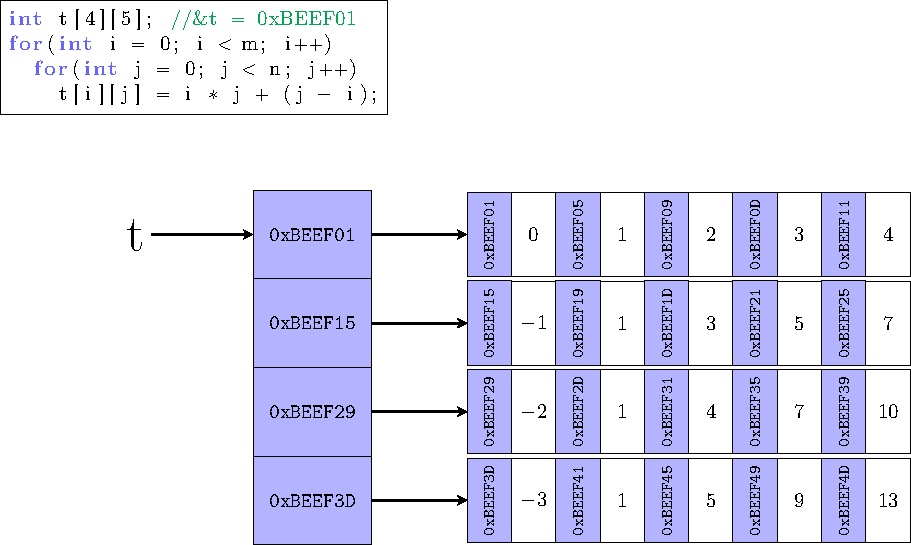
\includegraphics[height=5cm] {pics/tab.pdf}
\end{center}
\end{frame}

\begin{frame}
\frametitle{Question n° 1 : appel de \texttt{f(v)} (2/3)}
\begin{itemize}
\item Création de copie locale \texttt{v'} à l'appel
\end{itemize}
\begin{center}
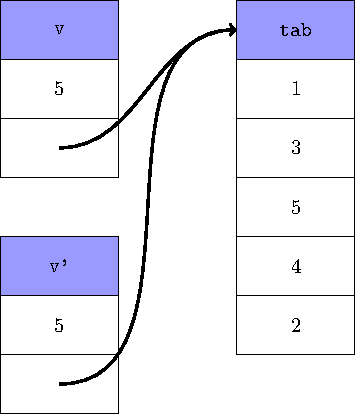
\includegraphics[height=5cm] {pics/tab2.pdf}
\end{center}
\end{frame}

\begin{frame}
\frametitle{Question n° 1 : appel de \texttt{f(v)} (3/3)}
\begin{itemize}
\item Destruction de copie locale \texttt{v'} en sortie de \texttt{f}
\end{itemize}
\begin{center}
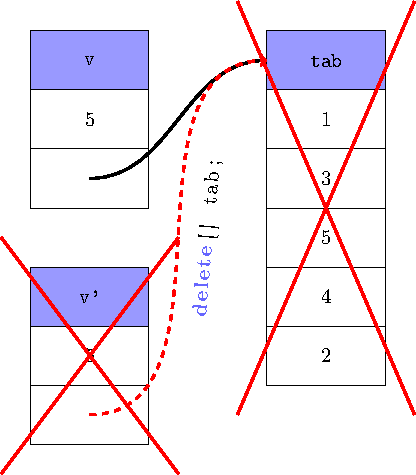
\includegraphics[height=5cm] {pics/tab3.pdf}
\end{center}
\end{frame}

\begin{frame}
\frametitle{Problèmes}
\begin{exampleblock}<+->{Observation}
	\begin{enumerate}[<+->]
	\item À l'appel, le vecteur \texttt{v} est copié, ainsi que l'adresse du tableau
		\begin{itemize}
		\item Pas la mémoire allouée sur le tas
		\end{itemize}	
	\item Quand la copie est détruite, le destructeur libère la mémoire
	\end{enumerate}
\end{exampleblock}
\begin{alertblock}<+->{Problème}
	\begin{itemize}[<+->]
	\item Le vecteur \texttt{v} est dans un état incohérent après l'appel
	\end{itemize}
\end{alertblock}
\begin{itemize}[<+->]
\item On ne veut peut-être pas utiliser \lstinline|shared_ptr|
	\begin{itemize}
	\item Effet de bord sur les copies
	\end{itemize}
\item Deux solutions possibles
	\begin{enumerate}
	\item Copie « manuelle »
	\item Empêcher la copie
	\end{enumerate}
\end{itemize}
\end{frame}

\begin{frame}
\frametitle{Copie « manuelle »}
\begin{itemize}[<+->]
\item Mise en œuvre via un constructeur de recopie
\item Écrire un constructeur de recopie qui copie manuellement les données allouées sur le tas
\end{itemize}
\begin{exampleblock}<+->{Avantages}
	\begin{itemize}[<+->]
	\item Copie fonctionnelle
	\end{itemize}
\end{exampleblock}
\begin{alertblock}<+->{Inconvénient}
	\begin{itemize}[<+->]
	\item Temps
	\item Mémoire
	\end{itemize}
\end{alertblock}
\end{frame}

\begin{frame}[containsverbatim]
\begin{itemize}
\item Fichier \texttt{vector-copy.cpp}
\end{itemize}
\begin{lstlisting}
class vector
{
	int n;
	double * tab;
	
	public:
		vector(int nbr) : n(nbr), tab(new double[n]) {}
		
		vector(const vector & v)
		{
			n = v.n;
			tab = new double[n];	
			for(int i = 0; i < n; i++)
				tab[i] = v.tab[i];		
		}
		
		~vector()
		{
			delete[] tab;
		}			

		double & operator [] (int i)
		{
			return tab[i];
		}		
};
\end{lstlisting}
\end{frame}

\begin{frame}
\frametitle{Copie interdite}
\begin{itemize}[<+->]
\item Mise en œuvre via un constructeur déclaré \lstinline|delete| (\cpp11)
	\begin{itemize}
	\item Pré \cpp11 : constructeur de recopie privé, ou déclaré mais pas implémenté
	\end{itemize}
\end{itemize}
\begin{exampleblock}<+->{Avantages}
	\begin{itemize}[<+->]
	\item Rapide
	\end{itemize}
\end{exampleblock}
\begin{alertblock}<+->{Inconvénient}
	\begin{itemize}[<+->]
	\item Peut-être pas ce qu'on veut
	\end{itemize}
\end{alertblock}
\end{frame}

\begin{frame}[containsverbatim]
\begin{itemize}
\item Fichier \texttt{vector-del.cpp}
\end{itemize}
\begin{lstlisting}
class vector
{
	int n;
	double * tab;
	
	public:
		vector(int nbr) : n(nbr), tab(new double[n]) {}
		
		vector(const vector & v) = delete;
		
		~vector()
		{
			delete[] tab;
		}			

		double & operator [] (int i)
		{
			return tab[i];
		}		
};
\end{lstlisting}
\begin{itemize}
\item Utiliser le passage par référence lors des appels de fonctions
\end{itemize}
\end{frame}

\begin{frame}
\frametitle{Question n° 2 : affectation de \texttt{v1} à \texttt{v2} (1/3)}
\begin{itemize}[<+->]
\item Instanciation des vecteurs \texttt{v1} et \texttt{v2}
\end{itemize}
\begin{center}
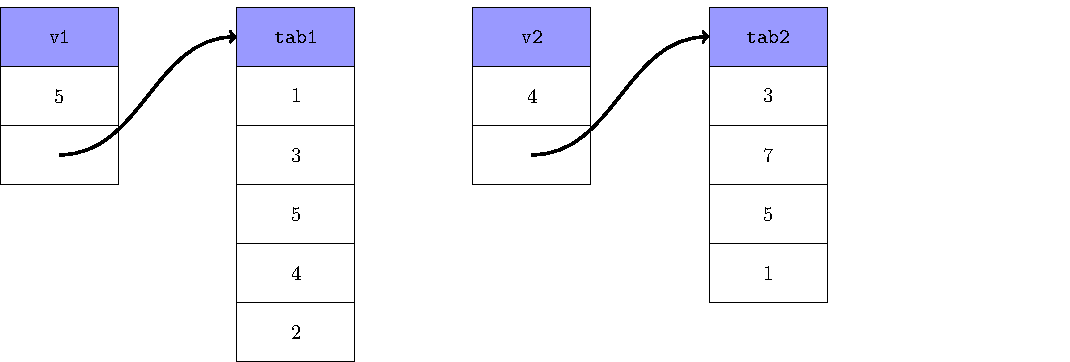
\includegraphics[height=4.5cm] {pics/aff.pdf}
\end{center}
\end{frame}

\begin{frame}
\frametitle{Question n° 2 : affectation de \texttt{v1} à \texttt{v2} (2/3)}
\begin{itemize}[<+->]
\item Affectation de \texttt{v1} à \texttt{v2}
\end{itemize}
\begin{center}
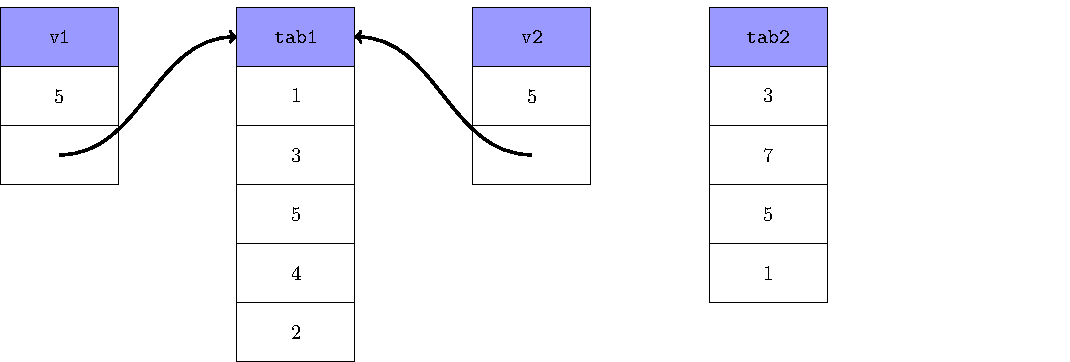
\includegraphics[height=4.5cm] {pics/aff2.pdf}
\end{center}
\end{frame}

\begin{frame}
\frametitle{Question n° 2 : affectation de \texttt{v1} à \texttt{v2} (3/3)}
\begin{itemize}[<+->]
\item Fuite mémoire : le tableau de \texttt{v2} n'a pas été détruit
\end{itemize}
\begin{center}
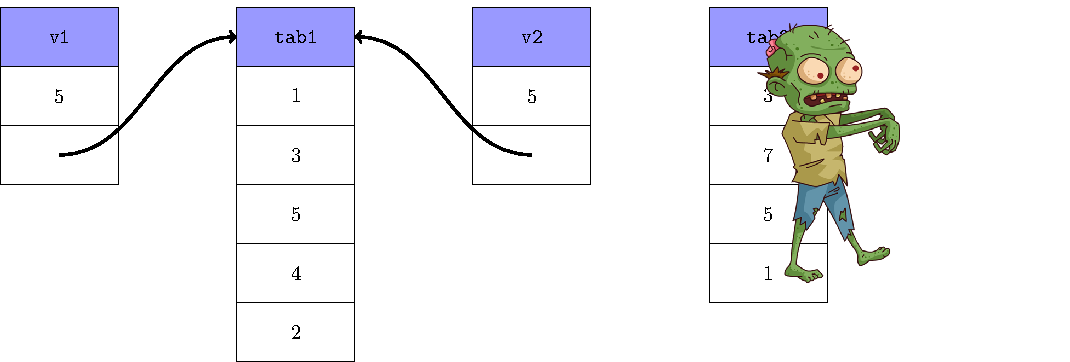
\includegraphics[height=4.5cm] {pics/aff3.pdf}
\end{center}
\end{frame}

\begin{frame}
\frametitle{Problèmes}
\begin{exampleblock}<+->{Observation}
	\begin{enumerate}[<+->]
	\item À l'affectation, le vecteur \texttt{v2} est affecté
		\begin{itemize}
		\item Les variables automatiques sont cohérentes
		\end{itemize}
	\item Quand la copie \texttt{v1} \emph{ou} \texttt{v2} sont détruits, \texttt{tab1} est libéré
		\begin{itemize}
		\item Pas \texttt{tab2}
		\end{itemize}
	\end{enumerate}
\end{exampleblock}
\begin{alertblock}<+->{Problème}
	\begin{itemize}[<+->]
	\item Fuite mémoire : \texttt{tab2} n'est pas désalloué
	\item Problème potentiel : double \lstinline|delete|
	\end{itemize}
\end{alertblock}
\begin{itemize}[<+->]
\item Deux solutions possibles
	\begin{enumerate}
	\item Affectation « manuelle » de « recopie »
	\item Empêcher l'affectation
	\end{enumerate}
\end{itemize}
\end{frame}

\begin{frame}
\frametitle{Affectation « manuelle »}
\begin{itemize}[<+->]
\item Mise en œuvre via surcharge de \texttt{=}
\item Écrire un opérateur \texttt{=} qui affecte et détruit manuellement les données allouées sur le tas
\end{itemize}
\begin{exampleblock}<+->{Avantages}
	\begin{itemize}[<+->]
	\item Affectation fonctionnelle
	\end{itemize}
\end{exampleblock}
\begin{alertblock}<+->{Inconvénient}
	\begin{itemize}[<+->]
	\item Temps
	\item Mémoire
	\item Complexité si ce n'est pas une recopie
	\end{itemize}
\end{alertblock}
\end{frame}

\begin{frame}[containsverbatim]
\begin{itemize}
\item Fichier \texttt{vector-copy.cpp}
\end{itemize}
\begin{lstlisting}
class vector
{
	int n;
	int count_affect;
	double * tab;
	
	public:
		vector(int nbr) : n(nbr), tab(new double[n]), count_affect(0) {}				
		
		~vector() { delete[] tab; }			
		
		vector& operator = (const vector& v)
		{
			if(this != &v) //check self-assign
			{
				delete tab;
				
				n = v.n;
				tab = new double[n];
				for(int i = 0; i < n; i++)
					tab[i] = v.tab[i];
			}
			return * this;
		}

		double & operator [] (int i)
		{
			return tab[i];
		}		
};
\end{lstlisting}
\end{frame}

\begin{frame}
\frametitle{Remarques}
\begin{itemize}[<+->]
\item Dans le cas de surcharge de \texttt{=}, comme on transmet le paramètre par référence, on doit le déclarer \lstinline|const| si on souhaite affecter un vecteur constant à un vecteur quelconque
\item On retourne le résultat de l'affectation par référence afin
	\begin{itemize}
	\item de pouvoir traiter les affectations multiples
	\item d'éviter d'appeler le constructeur de recopie
	\end{itemize}
\item Si on ne veut pas recopier les données à l'affectation
	\begin{enumerate}
	\item Création d'un attribut compteur d'affectations
	\item Le destructeur détruit \texttt{tab} si ce compteur est à zéro
	\item L'opérateur détruit \texttt{tab} si le compteur de \texttt{v} est à zéro
	\end{enumerate}	
\end{itemize}
\begin{block}<+->{Hygiène de programmation}
	\begin{itemize}[<+->]
	\item Ne faites pas de \lstinline|new|
	\end{itemize}
\end{block}
\end{frame}

\begin{frame}
\frametitle{Affectation interdite}
\begin{itemize}[<+->]
\item Mise en œuvre via un opérateur \texttt{=} déclaré \lstinline|delete| (\cpp11)
	\begin{itemize}
	\item Pré \cpp11 : opérateur d'affectation privé, ou déclaré mais pas implémenté
	\end{itemize}
\end{itemize}
\begin{exampleblock}<+->{Avantages}
	\begin{itemize}[<+->]
	\item Rapide
	\end{itemize}
\end{exampleblock}
\begin{alertblock}<+->{Inconvénient}
	\begin{itemize}[<+->]
	\item Peut-être pas ce qu'on veut
	\end{itemize}
\end{alertblock}
\end{frame}

\begin{frame}[containsverbatim]
\begin{itemize}
\item Fichier \texttt{vector-del.cpp}
\end{itemize}
\begin{lstlisting}
class vector
{
	int n;
	double * tab;
	
	public:
		vector(int nbr) : n(nbr), tab(new double[n]) {}				
		
		~vector()
		{
			delete[] tab;
		}
		
		vector& operator = (const vector& v) = delete;			

		double & operator [] (int i)
		{
			return tab[i];
		}		
};
\end{lstlisting}
\begin{itemize}
\item Construction possible, réaffectation impossible
	\begin{itemize}
	\item \lstinline|vector v(3, brol); //ok|
	\item \lstinline|vector v = vector(3, brol); //ko|
	\item \lstinline|v1 = v2; //ko|
	\end{itemize}
\end{itemize}
\end{frame}

\section{Littéraux définis par l'utilisateur}

\begin{frame}[containsverbatim]
\frametitle{Introduction}
\begin{itemize}
\item Supposons que l'on veuille modéliser le MRUA d'un point
\item À l'évidence, le code ci-dessous ne compile pas
\end{itemize}
\begin{lstlisting}
class MRUA
{
	double x0, t0, v0, a;
	
	public :
		MRUA(double x0 =0, double t0 = 0, double v0 = 0, double a = 9.81)
			: x0 ( x0 ) , t 0 ( t 0 ) , v0 ( v0 ) , a ( a )
		{}
		
		double operator () (double t_in_seconds) { ... }
		double operator () (double t_in_milliseconds) { ... }
};
\end{lstlisting}
\begin{itemize}
\item Il existe plusieurs techniques « standard » pour résoudre ce type d'ambiguïté
	\begin{itemize}
	\item Typage fort, tag dispatch, types fantômes, etc.
	\item Cf. Ch. 14
	\end{itemize}
\item En \cpp, dans ce cas précis, définir des littéraux dédiés est approprié
\end{itemize}
\end{frame}

\begin{frame}[containsverbatim]
\frametitle{Illustration}
\begin{itemize}
\item Fichier \texttt{mrua.cpp}
\end{itemize}
\begin{lstlisting}
class MRUA {
	long double x0, t0, v0, a;
	
	public :
		MRUA(long double x0 =0, long double t0 = 0, long double v0 = 0, long double a = 9.81)
			: x0 ( x0 ) , t0 ( t0 ) , v0 ( v0 ) , a ( a )
		{}
		
		long double operator () (long double t) { 
            long double dt = (t - t0);
            return x0 + v0 * dt + 0.5 * dt * dt;
        }
};

inline long double operator "" _ms(long double x) { return 0.001 * x; }
inline long double operator "" _s(long double x) { return x; }
inline long double operator "" _min(long double x) { return 60 * x; }
inline long double operator "" _h(long double x) { return 3600 * x; }

int main() {
    MRUA mrua;
    cout << "Position after 1 millisecond is " << mrua(1.0_ms) << " meters" << endl;
    cout << "Position after 1 second is " << mrua(1.0_s) << " meters" << endl;
    cout << "Position after 1 minute is " << mrua(1.0_min) << " meters" << endl;
    cout << "Position after 1 hour is " << mrua(1.0_h) << " meters" << endl;
}
\end{lstlisting}
\end{frame}

\begin{frame}
\frametitle{Contraintes}
\begin{enumerate}[<+->]
\item Les littéraux définis par l’utilisateur sont introduits par la surcharge
de l’opérateur \lstinline|""|
\item Le nom du littéral commence par '\texttt{\_}'
	\begin{itemize}
	\item La librairie standard se réserve les littéraux non préfixés
	\end{itemize}
\item Les paramètres ne peuvent être que de type \lstinline|const char*|, \lstinline|unsigned long long|, \lstinline|long double|, \lstinline|char|, «~\lstinline|const char*, size_t|~»
\item Les conversions implicites ne sont pas acceptées
	\begin{itemize}
	\item \texttt{mrua(1\_ms)} ne compile pas
	\end{itemize}
\item Pas de valeur par défaut
\end{enumerate}
\begin{exampleblock}<+->{Littéraux standards existants}
	\begin{itemize}[<+->]
	\item Dans \texttt{chrono.h}, les littéraux de durée \texttt{ns}, \texttt{us}, \texttt{ms}, \texttt{s}, \texttt{min}, \texttt{h} sont définis
	\item Dans \texttt{complex.h}, les littéraux imaginaires \texttt{if}, \texttt{il}, \texttt{i} sont définis 
	\end{itemize}
\end{exampleblock}
\end{frame}

\end{document}
